\section{Experiments} \label{sec:result}
\subsection{Experiment Setup}
We implemented the proposed CNT-Cache on gem5 simulator \cite{binkert2011gem5} 
and experimented on a multi-core processor with four Alpha 21264 cores. 
The main configurations of the processor are listed in Table\ref{tab:exp_setup}. 
The dynamic energy consumption of CNT-Cache is the accumulation of energy consumption 
of all the cache operations while the energy consumption of an cache operation 
is simulated with basic 9T-SRAM cell developed in \cite{CNFET2015model} using 
HSPICE with \SI{16}{nm} CNFET technology and the number of cache operations is 
obtained from the gem5 simulator. The CNT fabrication parameters used for 
the cache are presented in Table \ref{tab:CNT-parameter}. Finally, we selected 
8 programs from spec2006 and splash2 as a benchmark to evaluate the dynamic power 
consumption of CNT-Cache.

\begin{table}
    \centering
  \caption{Multi-core configuration}
  \label{tab:exp_setup}
  \begin{tabular}{ccccc}
    \toprule
      % Parameters & Setting \\
      \multirow{1}{*}{Freq.} &L1 I-Cache  &L1 D-Cache  &L2 Cache & Mem Lat.\\
    \midrule
      \multirow{3}{*}{3.3GHz} &64KB 2-way &64KB 2-way &16MB 8-way &\\
                &associative  &associative  &associative  &30 cycles\\
      %Core Frequency & 3.3GHz \\
      %L1 I-cache &64Kb 2-way associative\\
      %L1 D-cache &64Kb 2-way associative \\
      %L2 cache &16MB 8-way associative \\
      %Memory access latency & 30 cycles \\
  \bottomrule
\end{tabular}
\vspace{-1em}
\end{table}

\begin{table}
    \centering
    \caption{CNT Parameters\cite{sun2017high}}
    \label{tab:CNT-parameter}
    \begin{tabular}{cccccc}
      \toprule
        \multirow{3}{*}{Pitch} &Gate &CNT &Prob of &Prob of  &Prob of\\
                &width &Diameter &m-CNT &removed &removed\\
                &  &  &  &m-CNT & s-CNT\\
      \midrule
        5.3nm &16nm &0.84nm &5\%  &99.99\%  &2.5\% \\
      \bottomrule
    \end{tabular}
\vspace{-1em}
\end{table}

\subsection{Experiment results}
CNT-Cache is designed to improve the energy efficiency of CNFET-based cache architecture with 
runtime cache line encoding. It relies on accurate cache access pattern prediction to 
decide an appropriate encoding direction. To evaluate the proposed adaptive encoding, 
we compare the energy consumption of CNT-Cache and the one using optimal cache line encoding.
Note that we extract the cache access trace and determine the optimal cache encoding for each 
encoding window i.e. the number of cache accesses that CNT-Cache conducts a prediction. 
Meanwhile, we also compare CNT-Cache with a baseline CNFET-based cache. 

In the experiment, the window is set to 15 and the cache line is encoded without partition. 
Figure \ref{fig:compare} exhibits that the proposed CNT-Cache decreases the energy 
consumption by 22.2\% on average compared to the baseline design and it incurs little 
runtime penalty. As the magnitude of energy saving and runtime penalty differs 
dramatically, the energy efficiency i.e. energy delay product of CNT-Cache is roughly 
determined by its energy consumption. Particularly, for the lib program, the encoding is typically valid 
for much longer time and CNT-Cache saves up to 46.6\% energy. In contrast, the largest runtime 
penalty is around 0.5\% in gro program. It shows that CNT-Cache has little influence on 
the performance of the benchmark programs. Thus, we will focus on the energy consumption 
analysis in the rest of the experiments. When compared to CNT-Cache 
with optimal encoding, the energy consumption of CNT-Cache is around 8\% higher on average, 
which is mainly caused by the penalty of false cache line predictions. 

\begin{figure}
	% \center{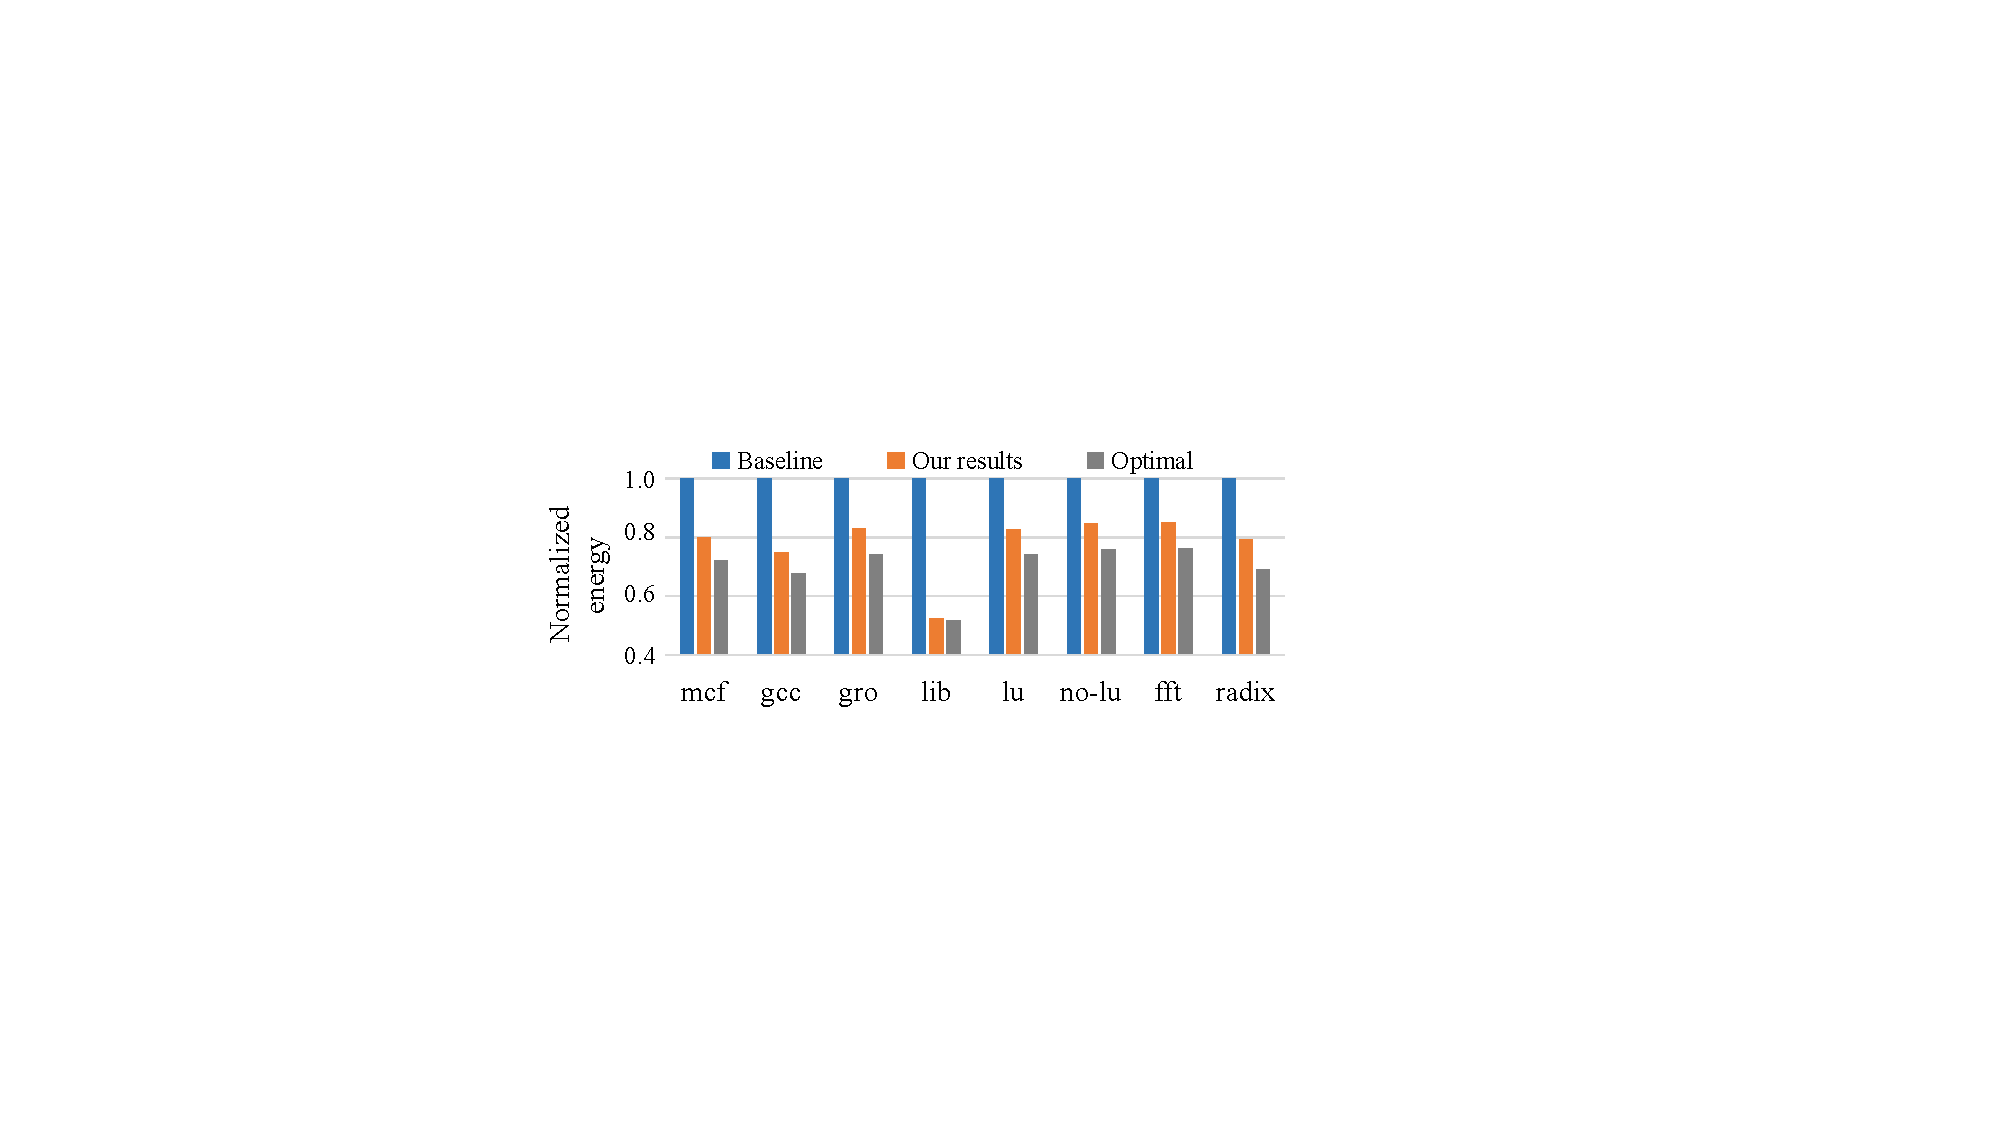
\includegraphics[width=0.95\linewidth]{compare}}
	\center{}
	\subfigure[Energy consumption]{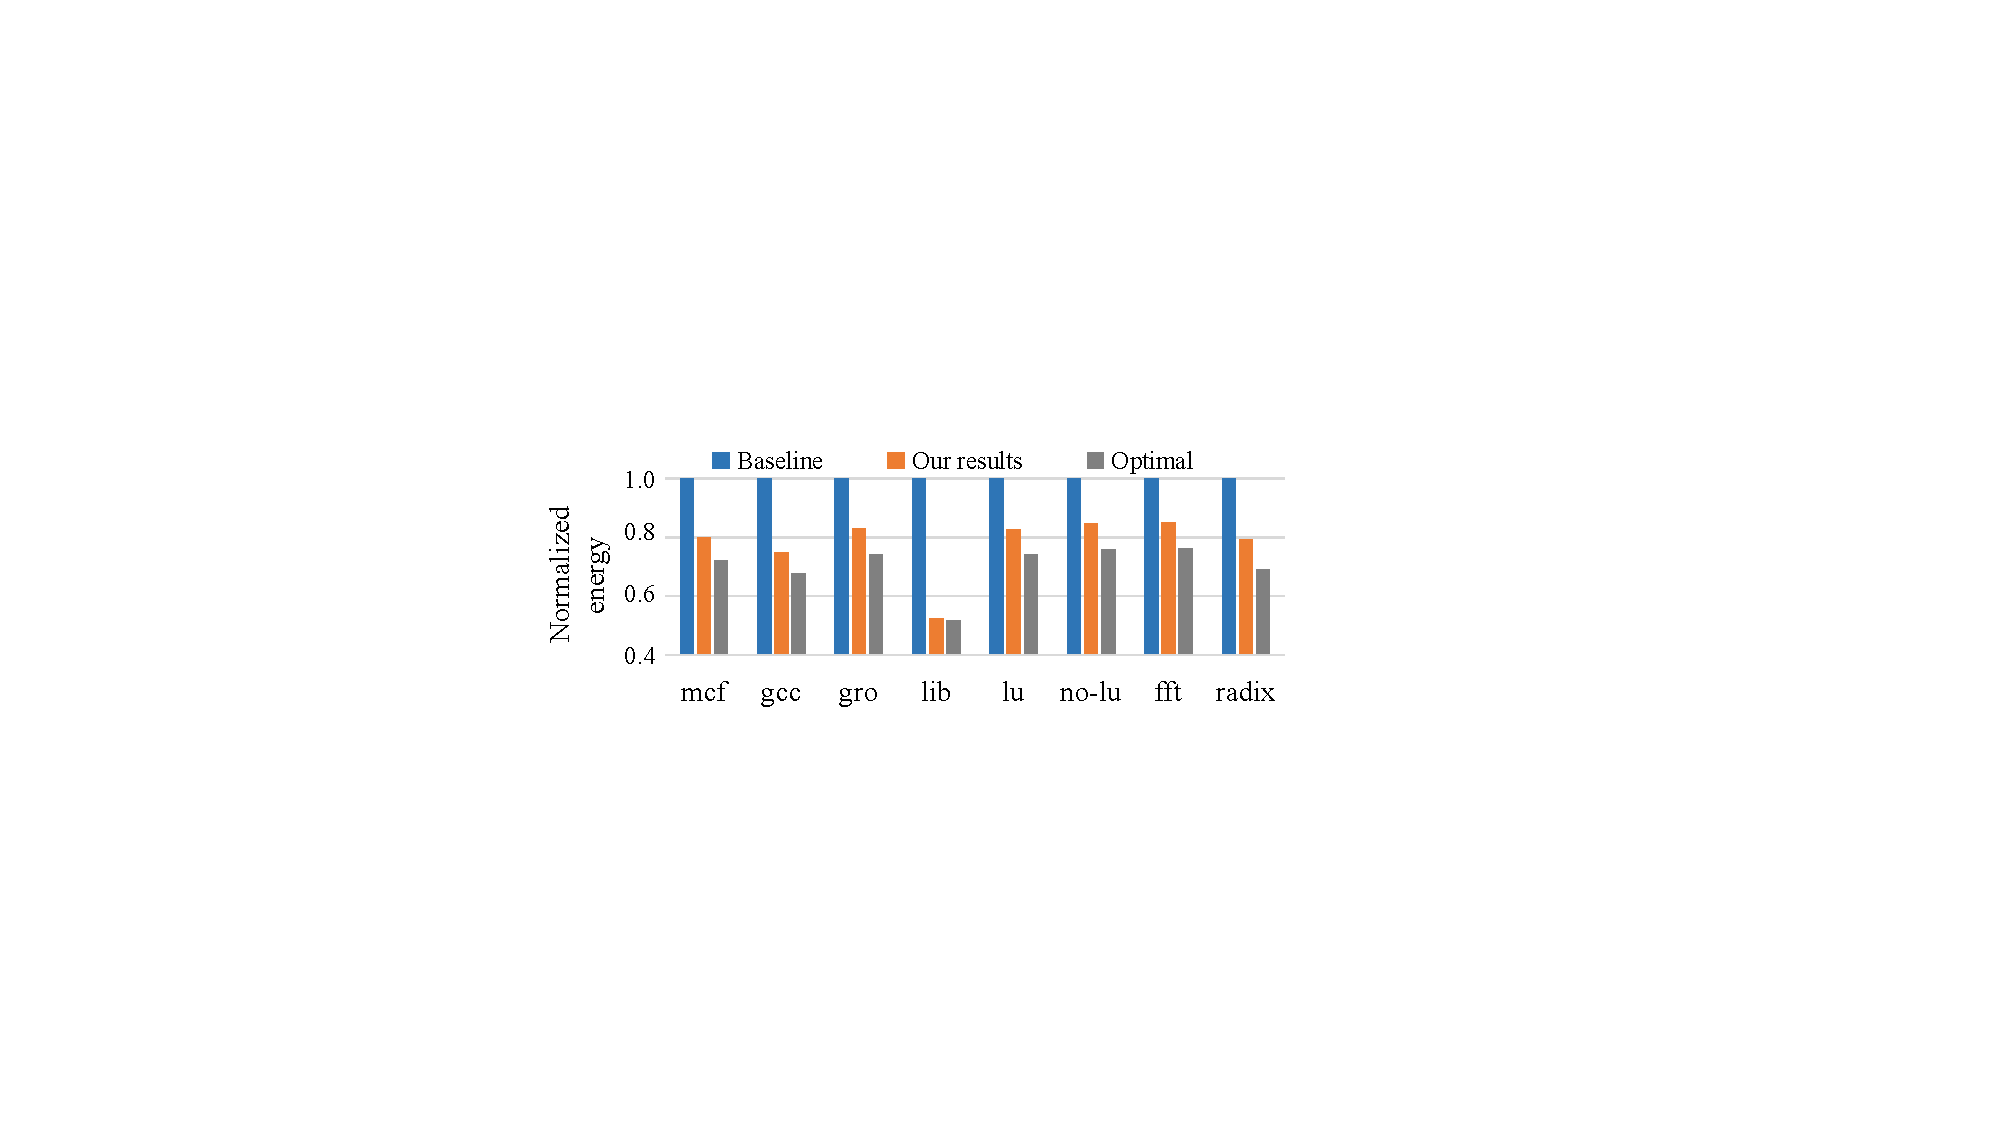
\includegraphics[width=0.85\linewidth]{compare}}
	\subfigure[Runtime]{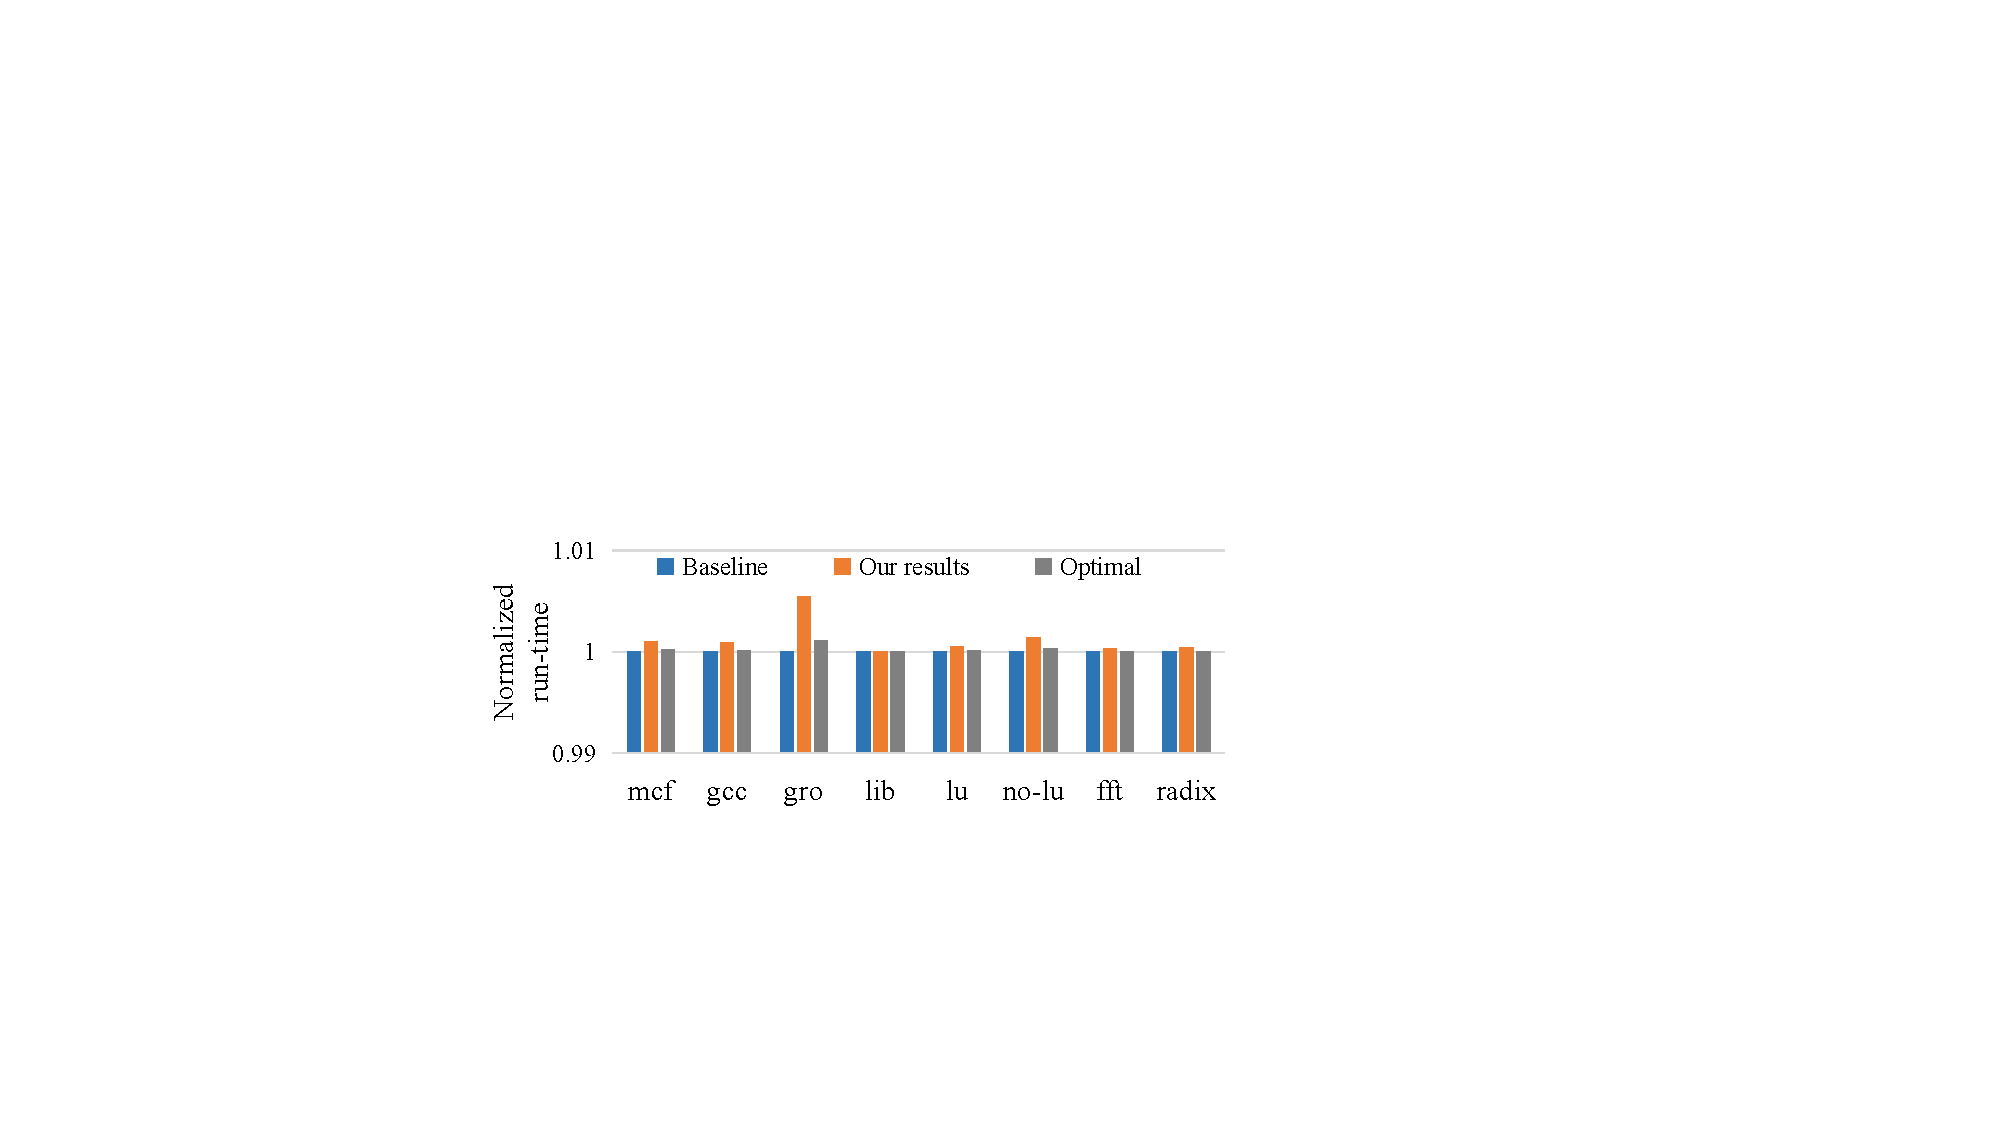
\includegraphics[width=0.85\linewidth]{cmp_delay}}
	\caption{Energy consumption and runtime comparison among the baseline design, 
	the proposed CNT-Cache design and CNT-Cache with optimal encoding}
\label{fig:compare}
\vspace{-1.5em}
\end{figure}

%As mentioned, the window size is an important design parameter of CNT-Cache. 
%Figure \ref{fig:windows} shows the energy consumption distribution of CNT-Cache with different 
%window sizes. The energy consumption of CNT-Cache roughly consists of three parts including 
%energy consumption of the baseline cache architecture (base), energy consumption of the 
%increased cache cell (Increased Cell), and energy consumption of the run-time encoding (Encoding).
%'Base' refers to the basic cache structure in CNT-Cache. 'Increased cell' refers to the 
%direction bits and the access history bits added to each cache line. 
%'Encoding' includes both the prediction logic and the encoding logic, but its encoding energy 
%consumption involves energy consumption of the relevant logic as well as the energy consumption 
%of the additional cache line update when the encoding direction is changed.
%When the encoding windows increases from 3 to 31, the energy consumption of 'Encoding' reduced 
%due to less encoding switch. Nevertheless, the energy consumption of 'Base' and 'increased cell' 
%increased gets larger. Taking all the influence into consideration, $W=15$ works best in general 
%and is utilized in the rest of the experiments.

%\begin{figure}
%    \center{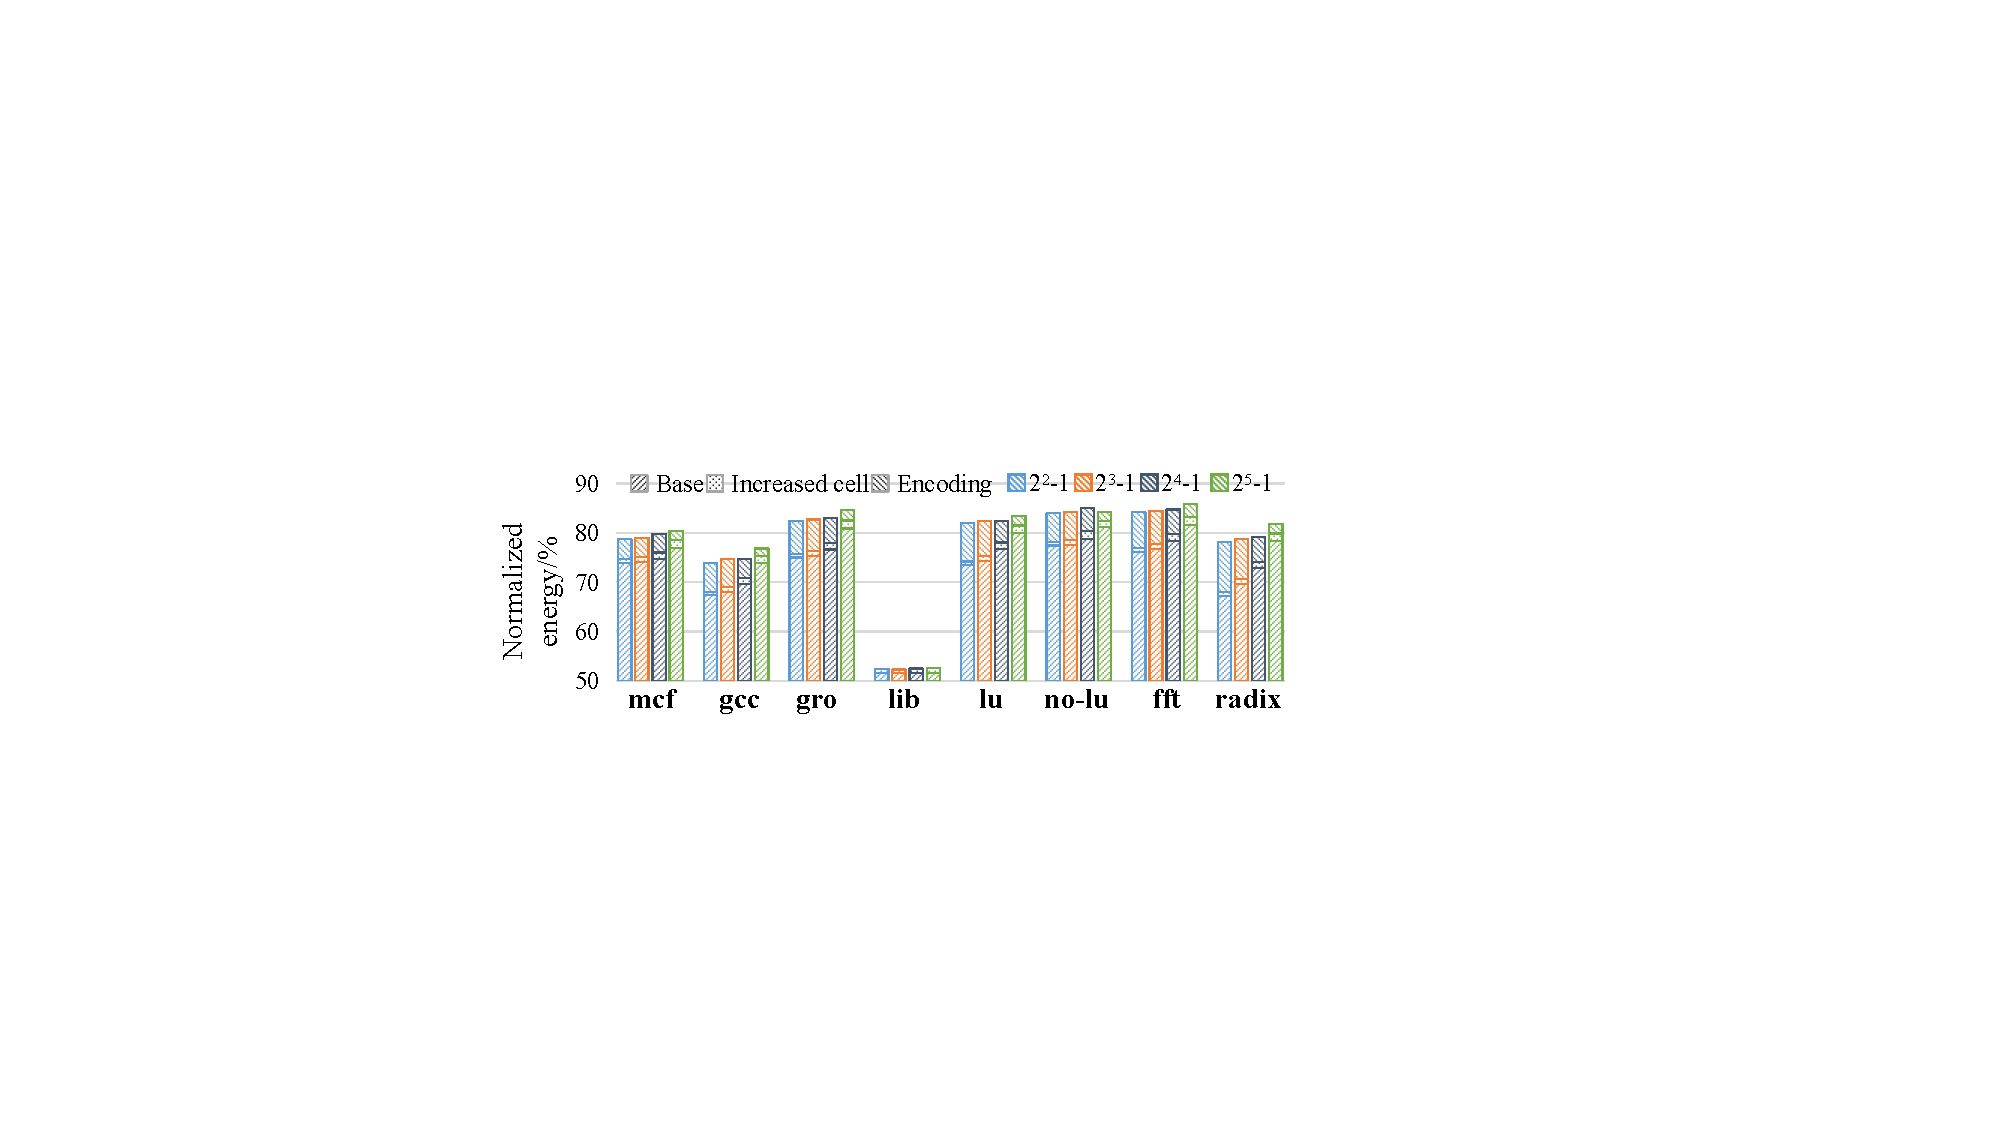
\includegraphics[width=0.95\linewidth]{windows}}
%    \caption{Influence of window size on CNT-Cache energy consumption}
%    \label{fig:windows}
%\vspace{-1em}
%\end{figure}

As mentioned in Section \ref{sec:warp}, the encoding granularity and the 
prediction threshold are the most critical parameters that affect the 
energy consumption of CNT-Cache. To gain insight of CNT-Cache energy consumption, 
we further explore the influence of the two parameters. 
Figure \ref{fig:encoding-granularity} shows the energy consumption distribution 
of CNT-Cache with different encoding granularity.
The energy consumption of CNT-Cache roughly consists of three parts including 
energy consumption of the baseline cache architecture (base), energy consumption of the 
increased cache cell (Increased Cell), and energy consumption of the run-time encoding (Encoding).
'Base' refers to the basic cache structure in CNT-Cache. 'Increased cell' refers to the 
direction bits and the access history bits added to each cache line. 
'Encoding' includes both the prediction logic and the encoding logic, but its encoding energy 
consumption involves energy consumption of the relevant logic as well as the energy consumption 
of the additional cache line update when the encoding direction is changed.
As shown in the figure, when the encoding granularity changes from 64B to 2B, 
more bits of the cache are changed to be more energy efficient to cache operations. 
Nevertheless, the direction bit number increases from 1 
to 32 and more SRAM cells are required accordingly. As shown in the Figure, the increased energy 
consumption of the cells becomes larger than energy saving on baseline cache architecture.
The encoding energy consumption that is mostly induced by the additional cache line data update 
increases slightly. In this case, we find that coarse encoding granularity is preferred in general.

\begin{figure}
    \center{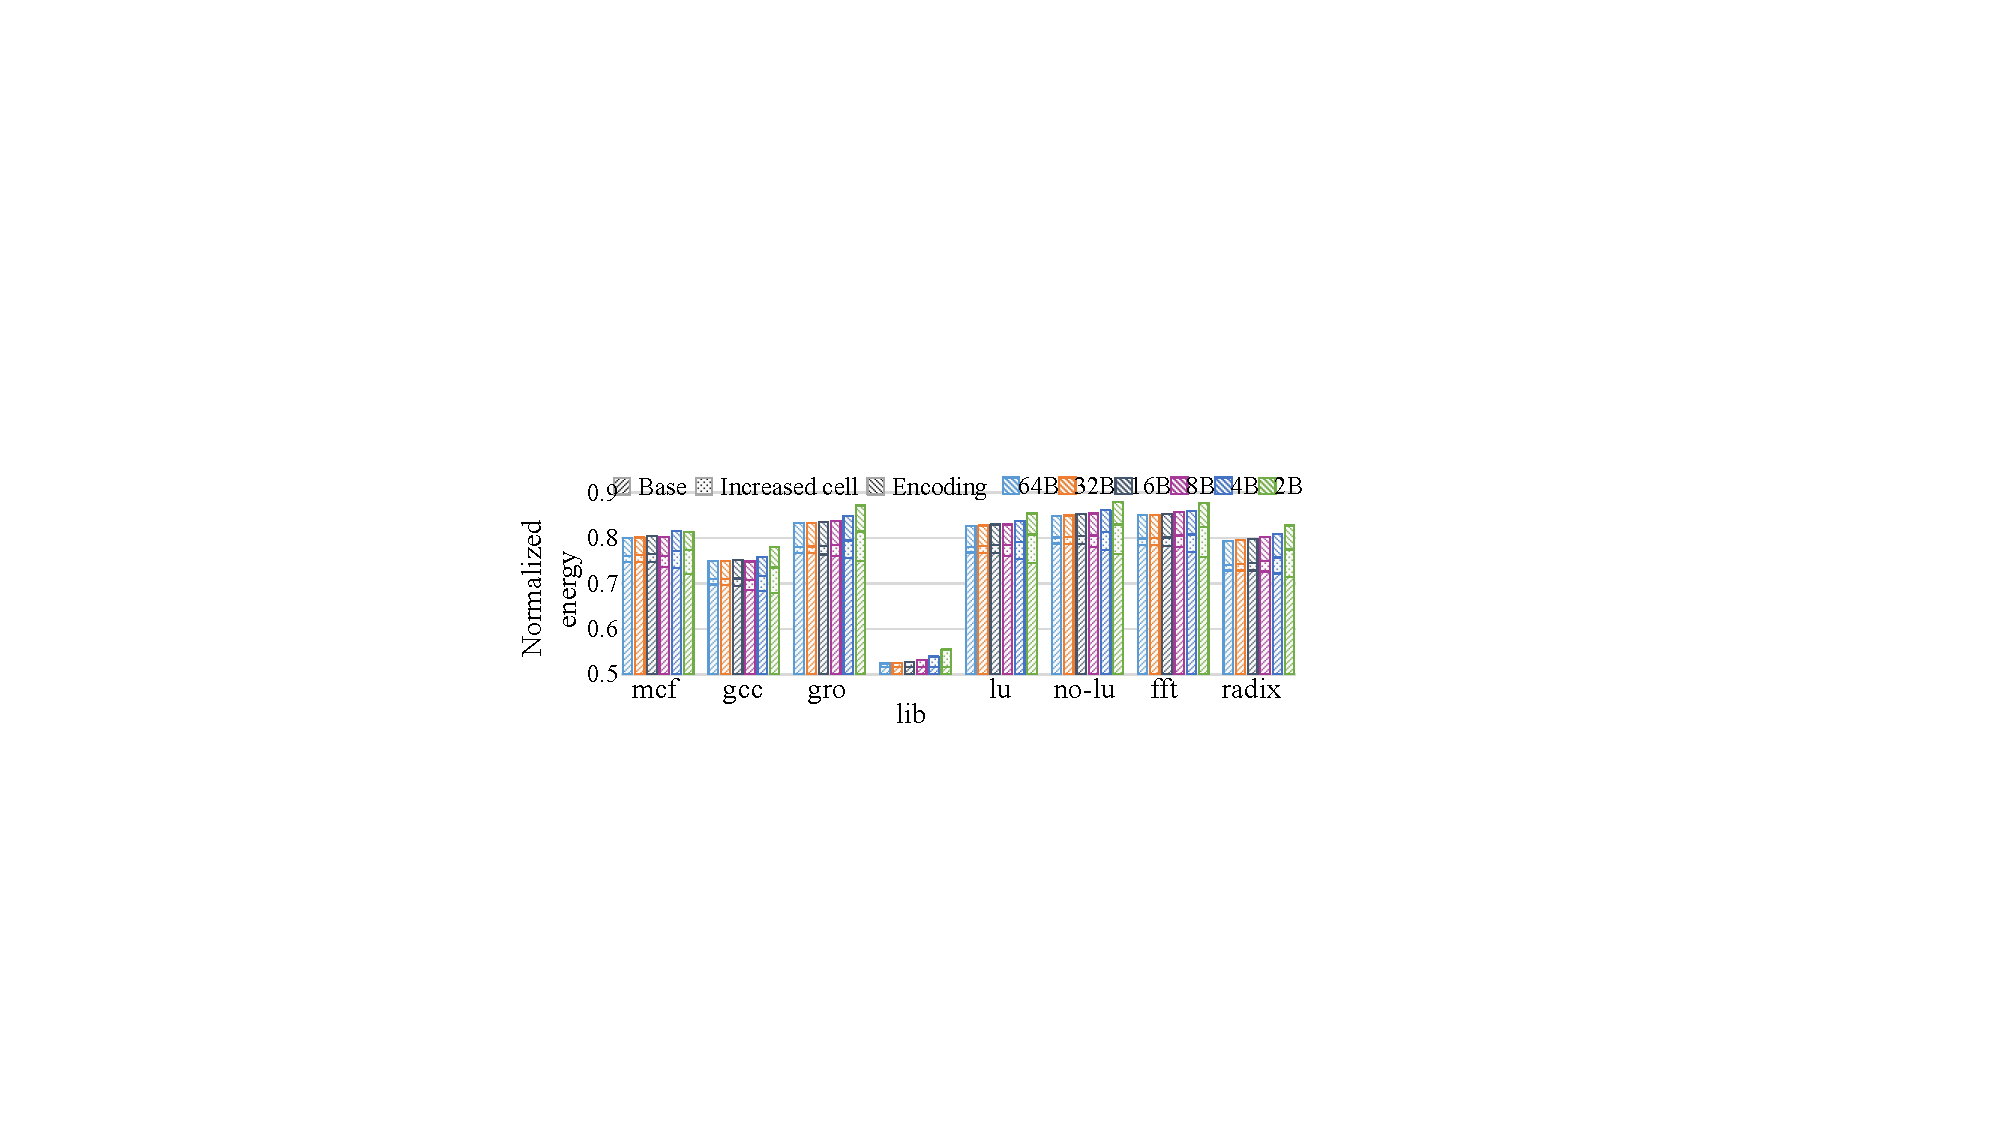
\includegraphics[width=0.99\linewidth]{gran}}
    %\center
    %    \subfigure[]{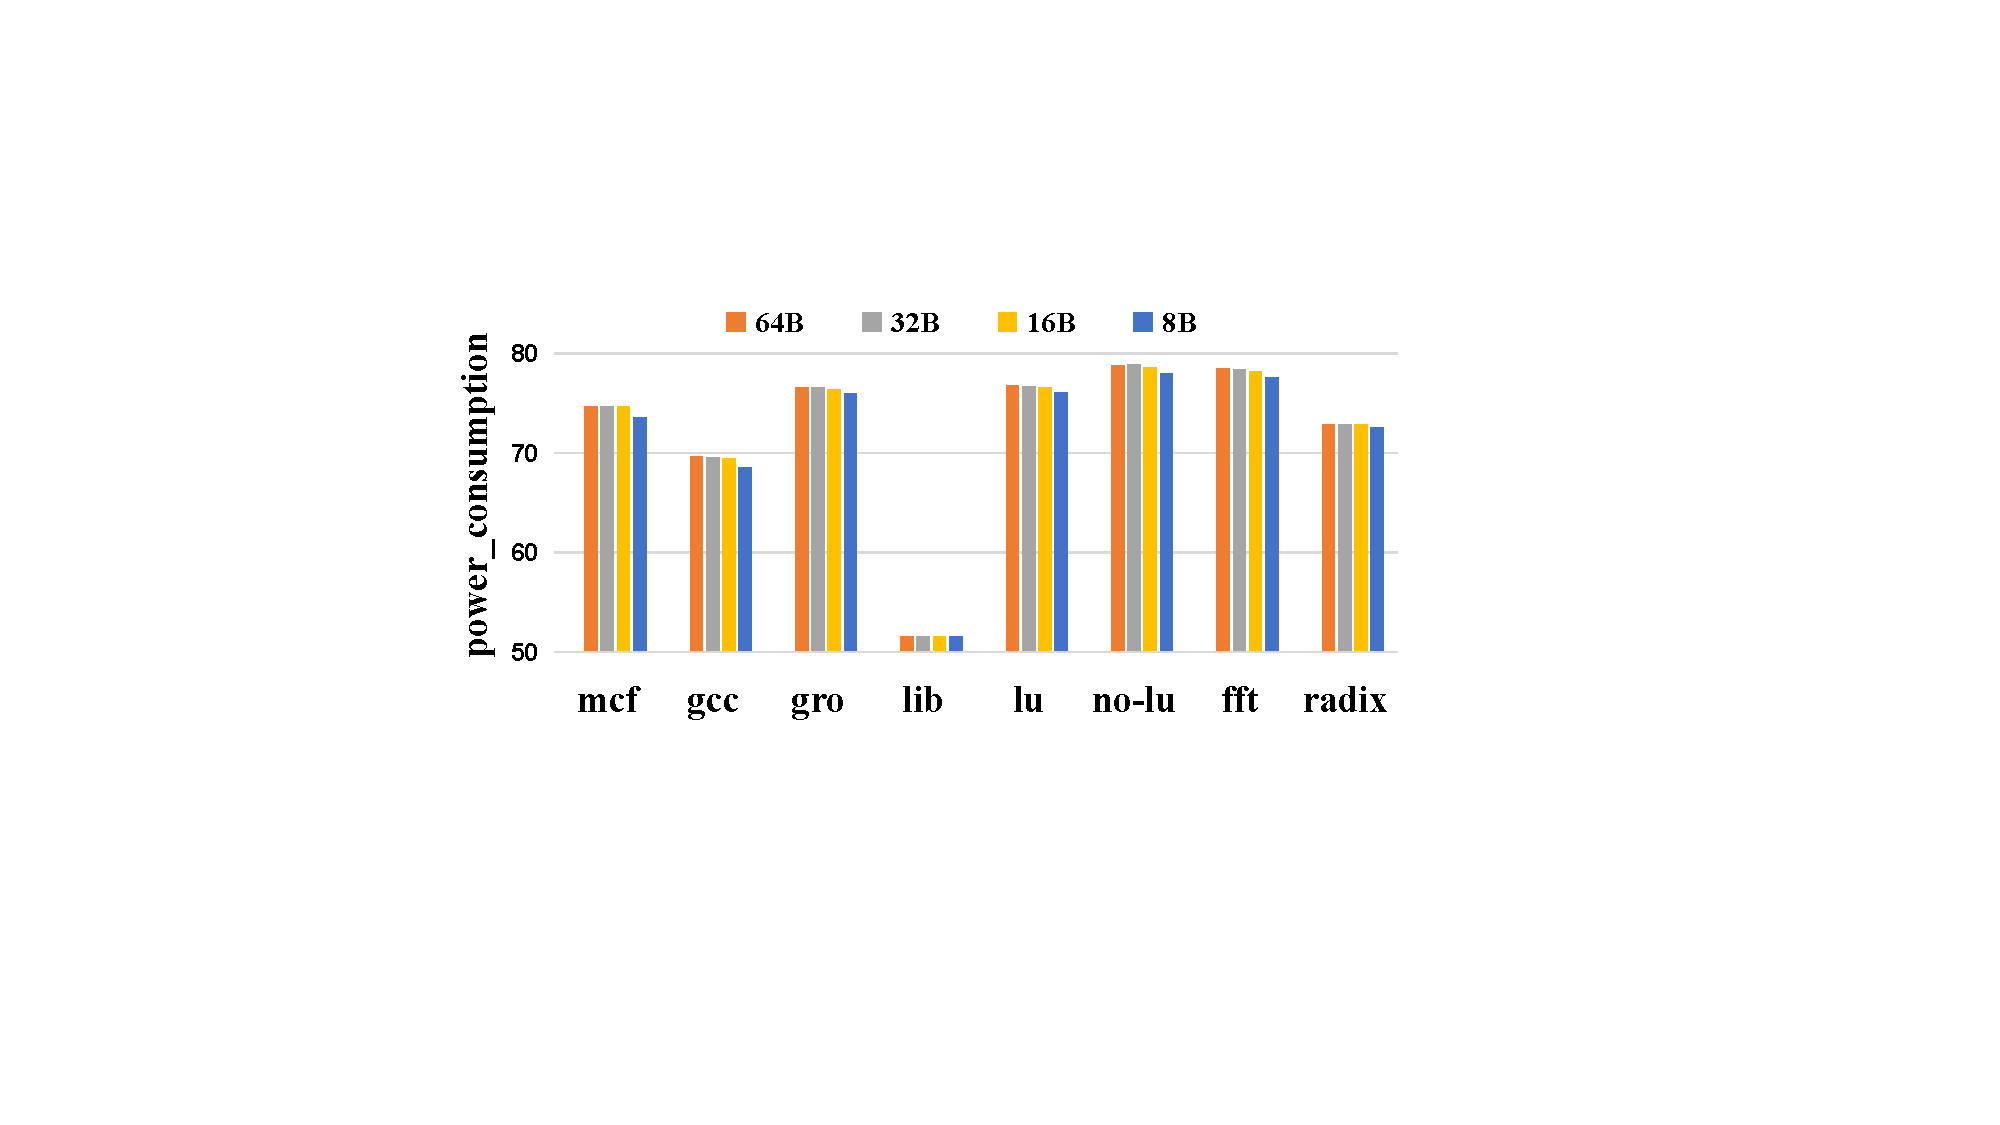
\includegraphics[width=0.92\linewidth]{gran_a}}
    %    \subfigure[]{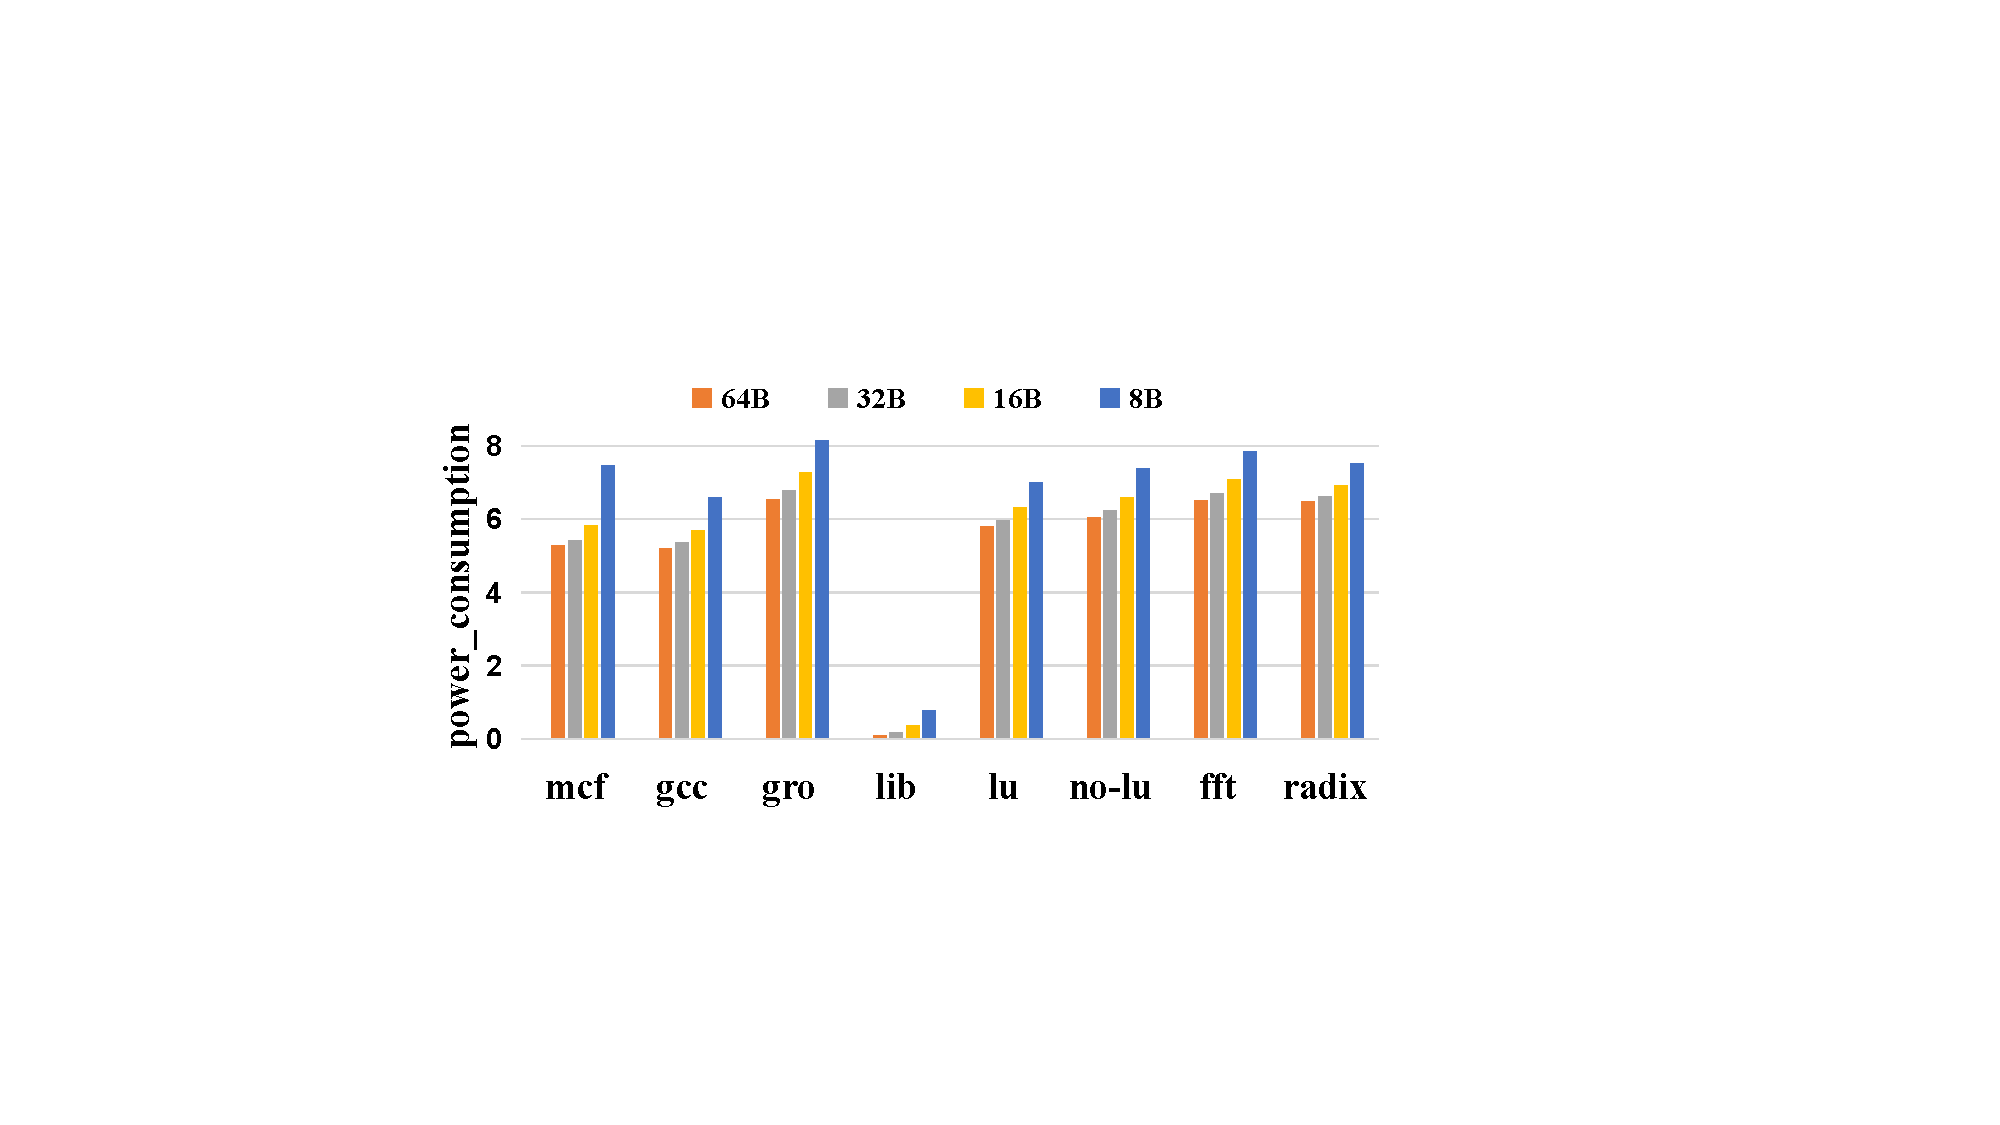
\includegraphics[width=0.92\linewidth]{gran_b}}
    %    \subfigure[]{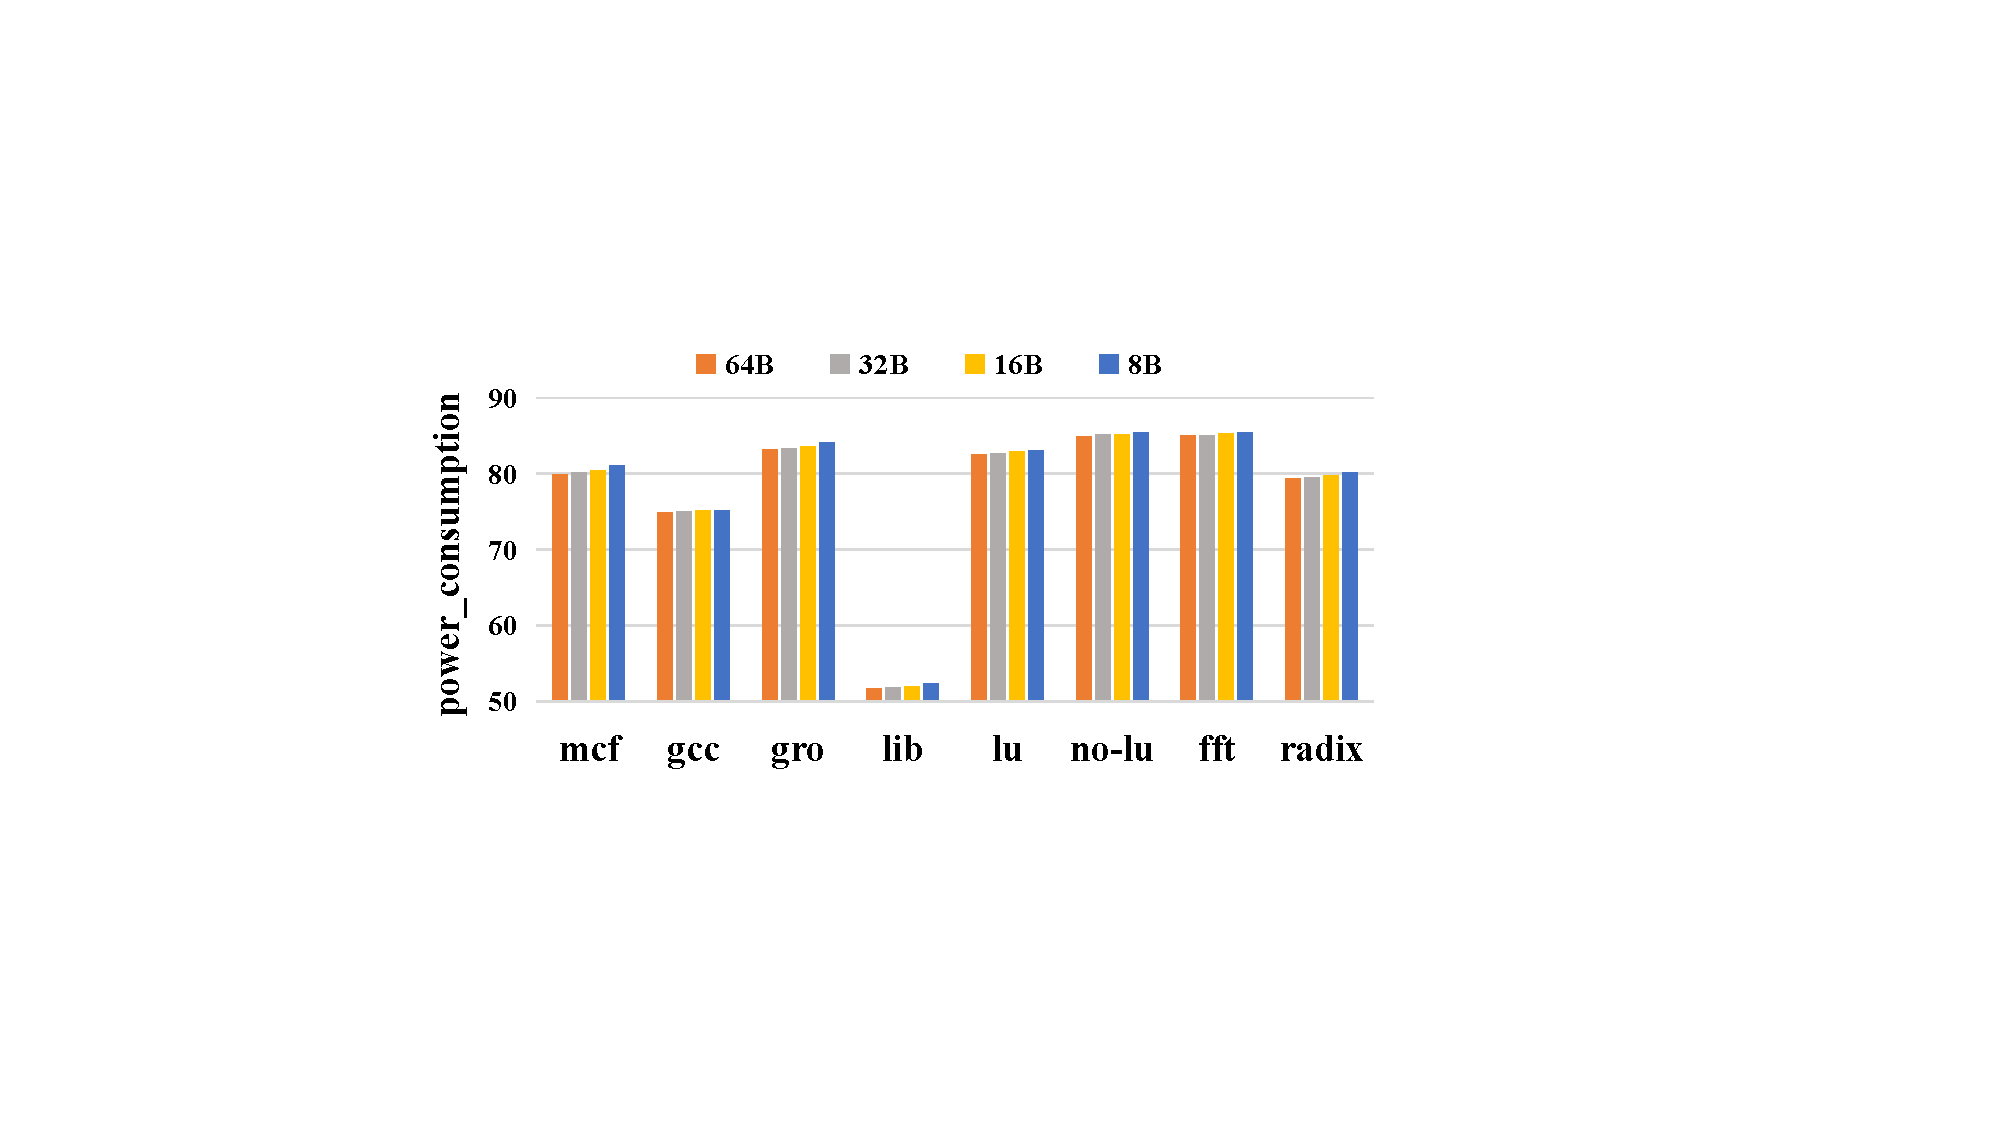
\includegraphics[width=0.92\linewidth]{gran_c}}
    \caption{CNT-Cache energy consumption distribution with different encoding granularity. 
    The granularity ranges from 64B, 32B, 16B, 8B, 4B to 2B.}
\label{fig:encoding-granularity}
\vspace{-1em}
\end{figure}

Another key design parameter is the bit number threshold used in the 
encoding direction predictor. Basically, larger threshold indicates 
more strict encoding direction switch, which avoids the encoding with 
trivial energy saving. We increase the threshold by 0\%, 5\%, 10\%, 
15\% and 20\% respectively. As shown in Figure \ref{fig:threshold-inc}, it can be observed that 
the threshold calculated with the analytical model works for most of 
the benchmarks and it squeezes sufficient energy saving. Still, more 
energy saving is gained with higher threshold in $mcf$ and gro. 
This is mainly caused by the dramatically reduced encoding 
overhead as shown in the Figure. $mcf$ is used to address network flow problems 
and involves a lot of irregular cache accesses. Thus, the cache line access 
pattern (read/write intensive) may change frequently and there are more 
borderline encoding switch. In this case, increased threshold is 
beneficial.

\begin{figure}
    \center{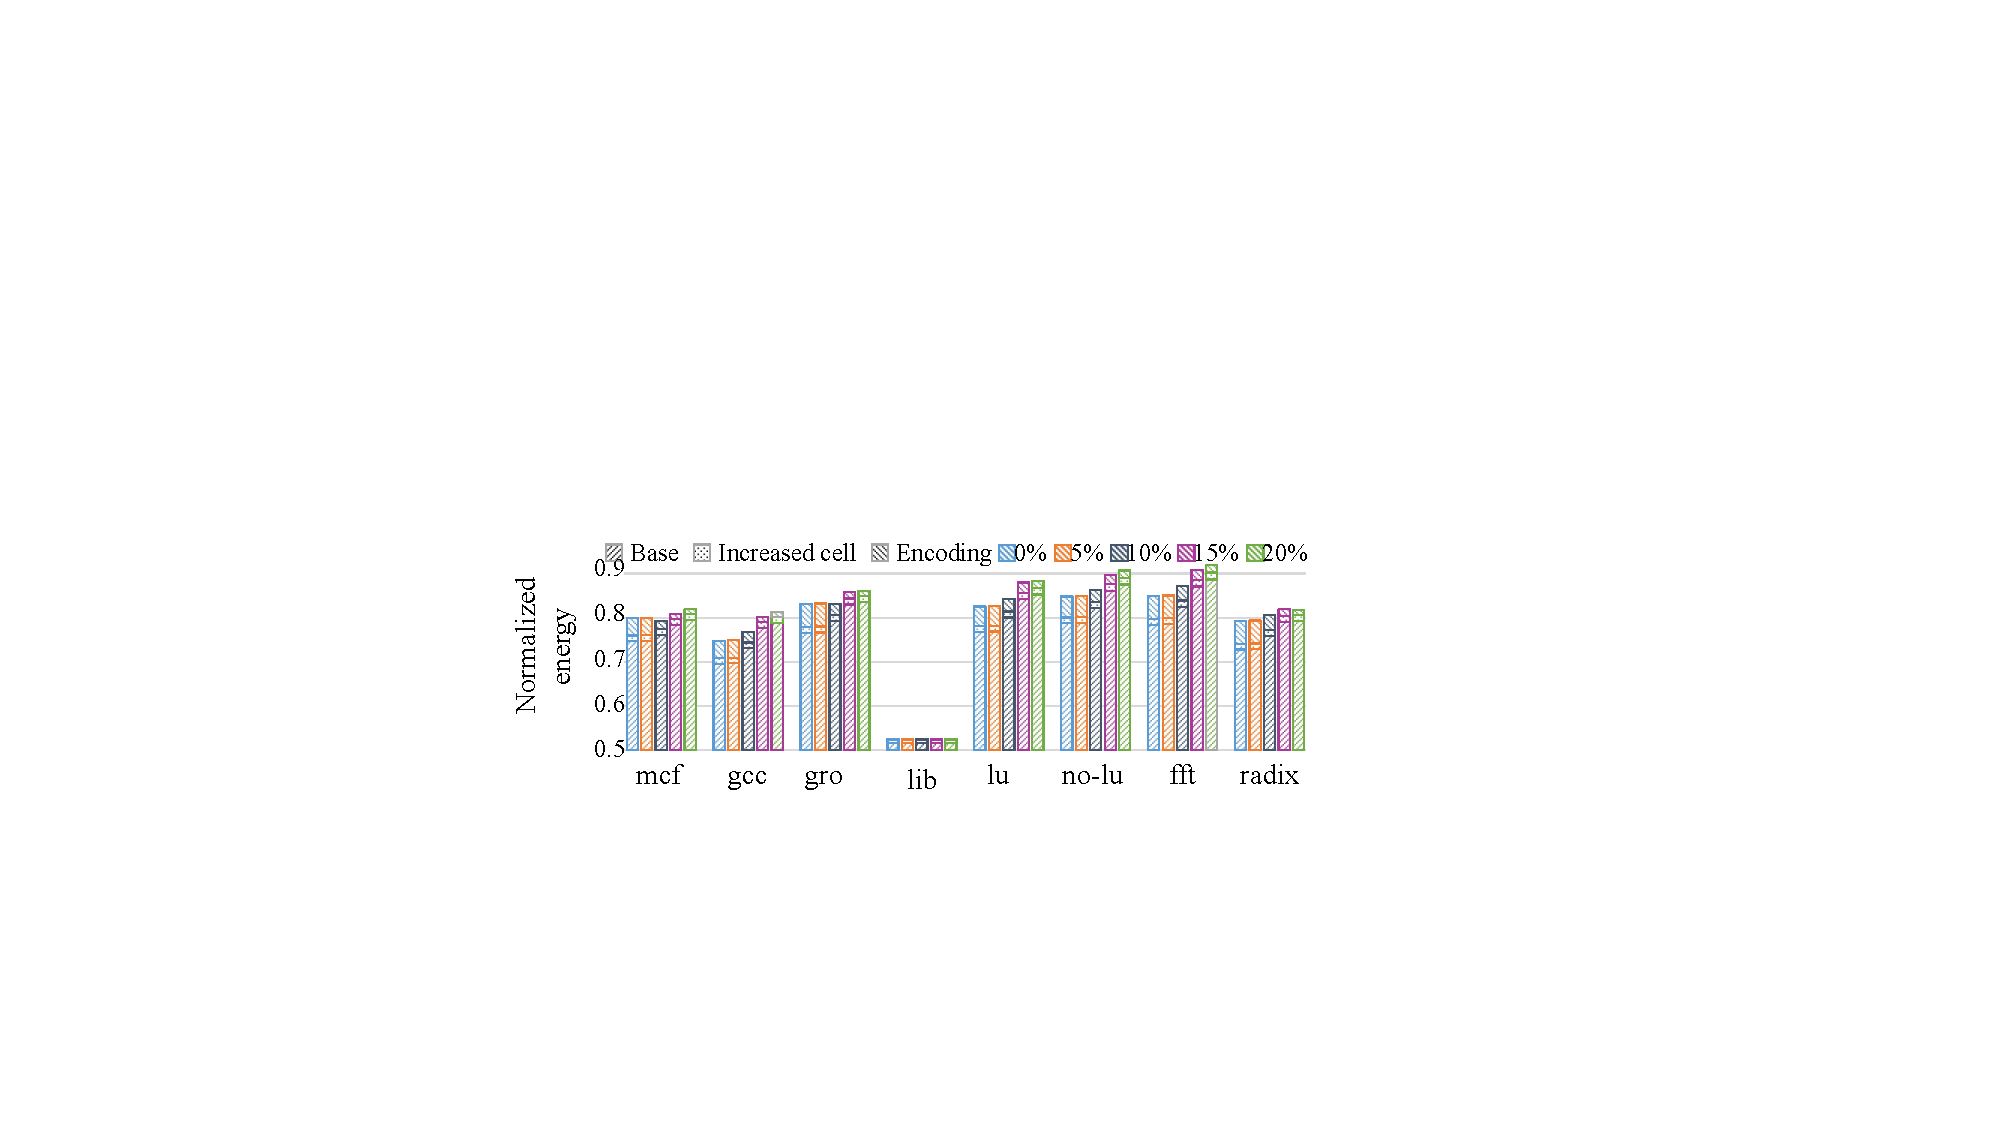
\includegraphics[width=0.99\linewidth]{thes}}
    %\center 
    %    \subfigure[]{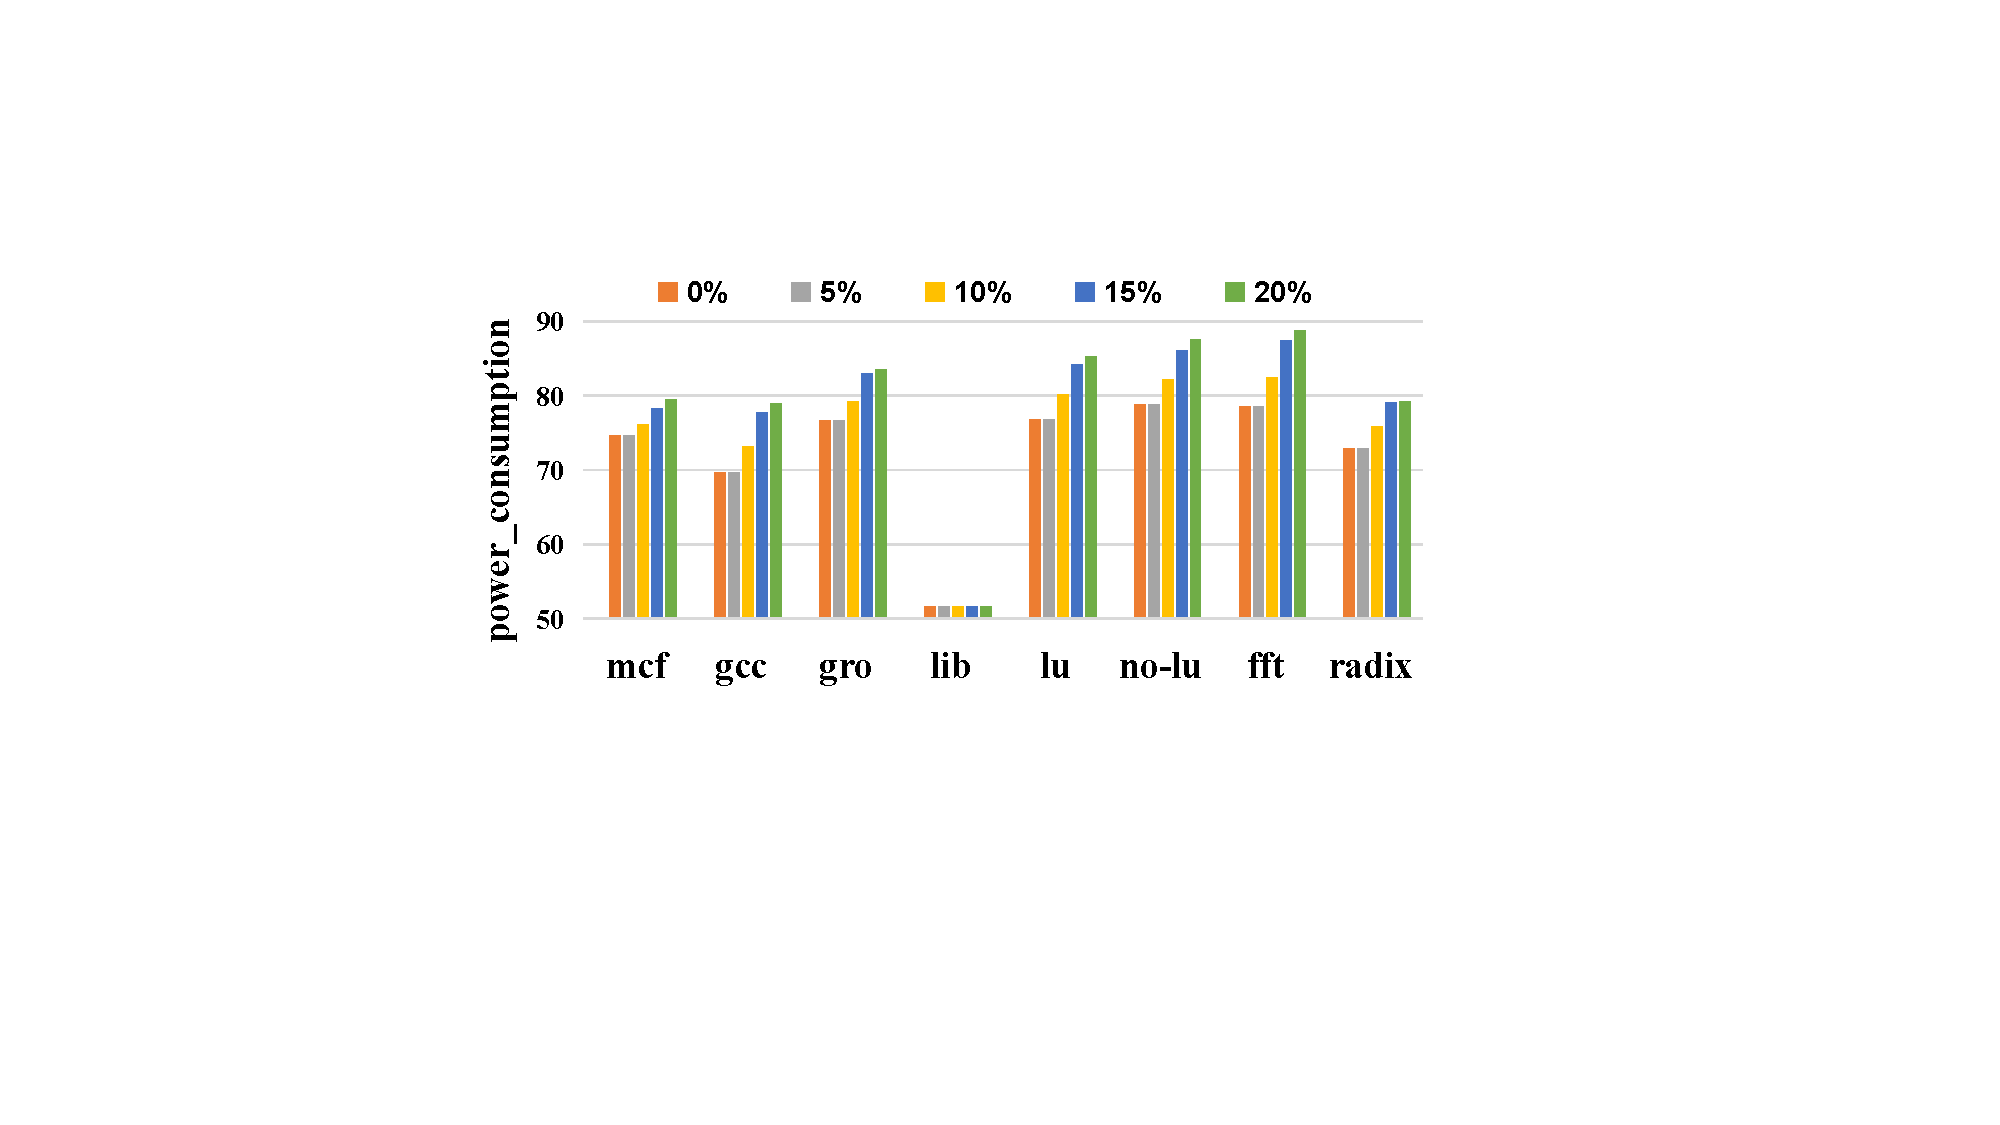
\includegraphics[width=0.92\linewidth]{thes_a}}
    %    \subfigure[]{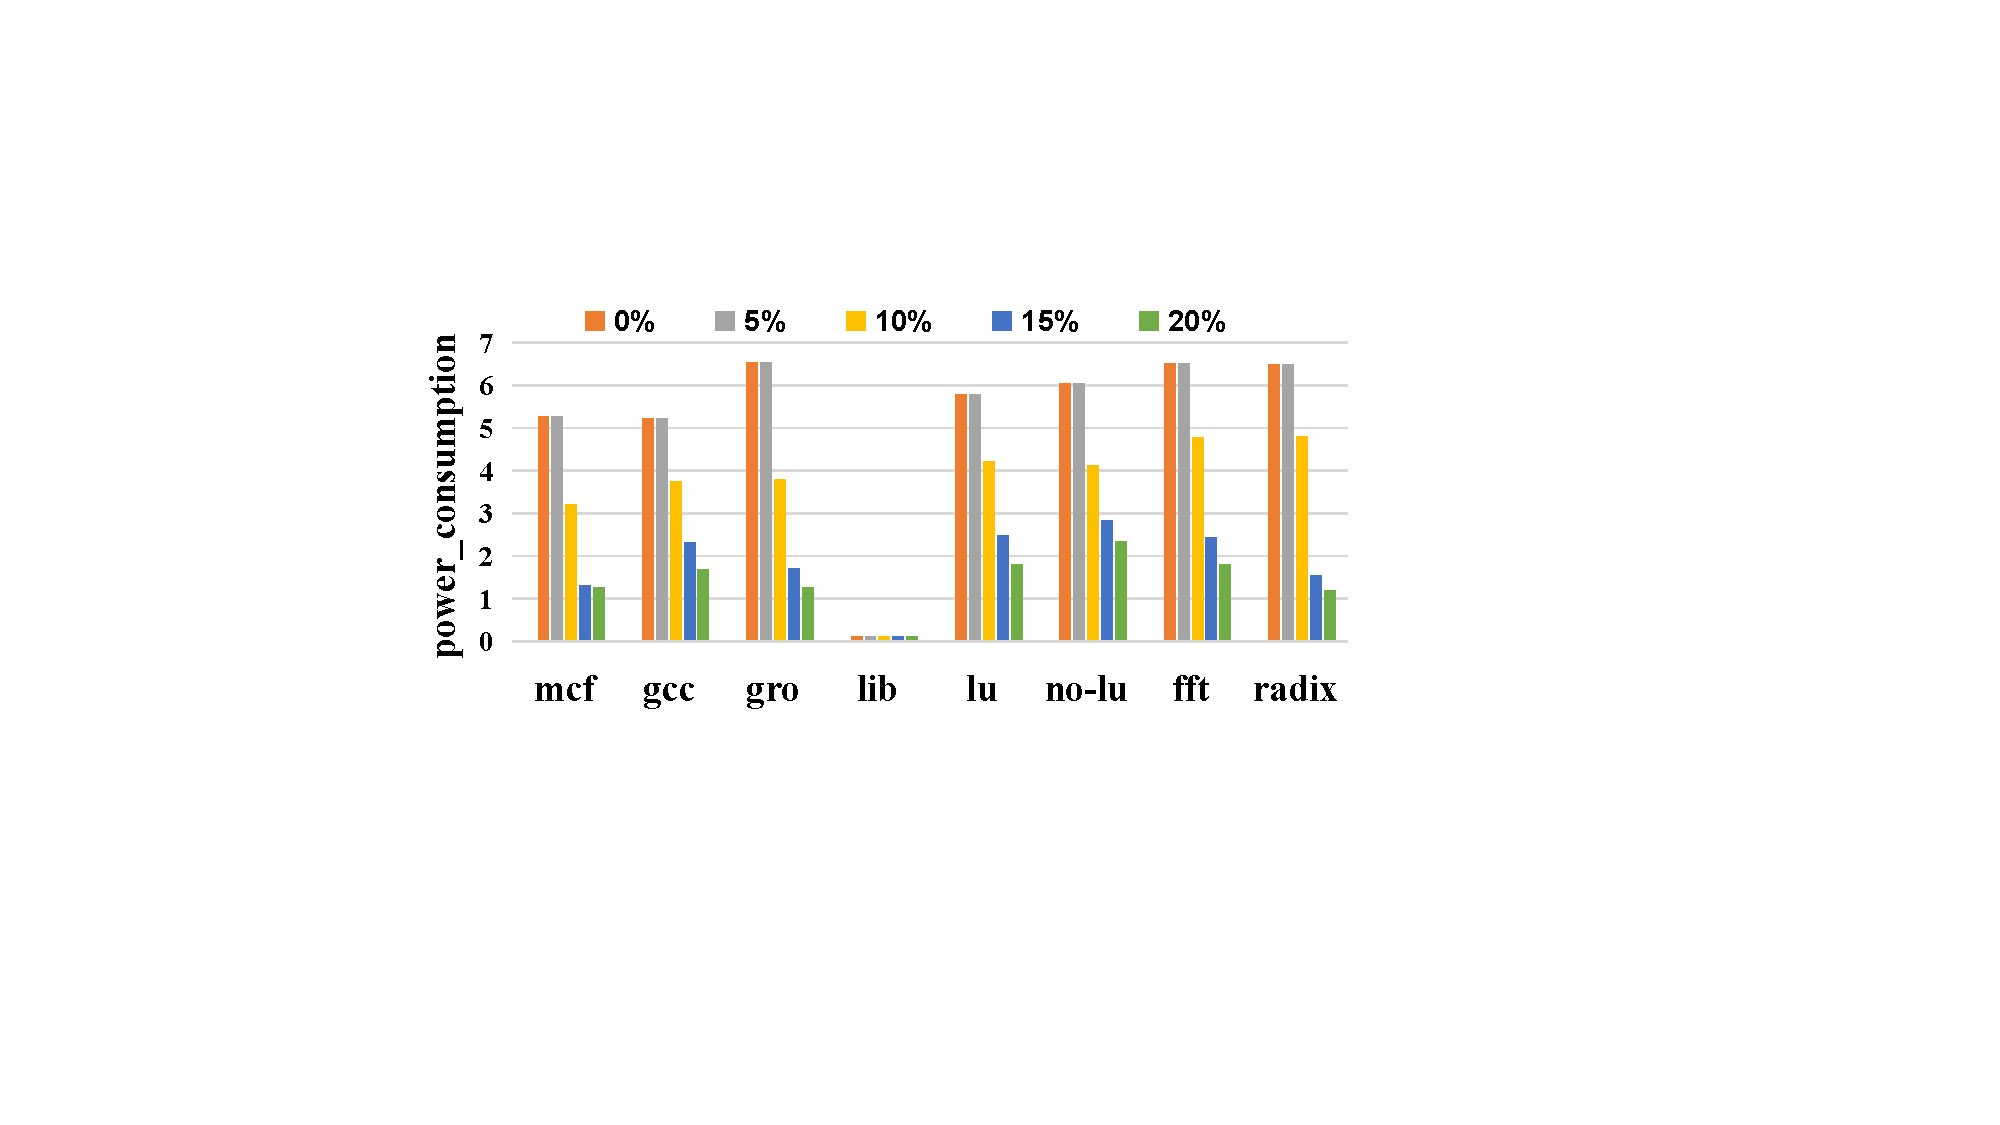
\includegraphics[width=0.92\linewidth]{thes_b}}
    %    \subfigure[]{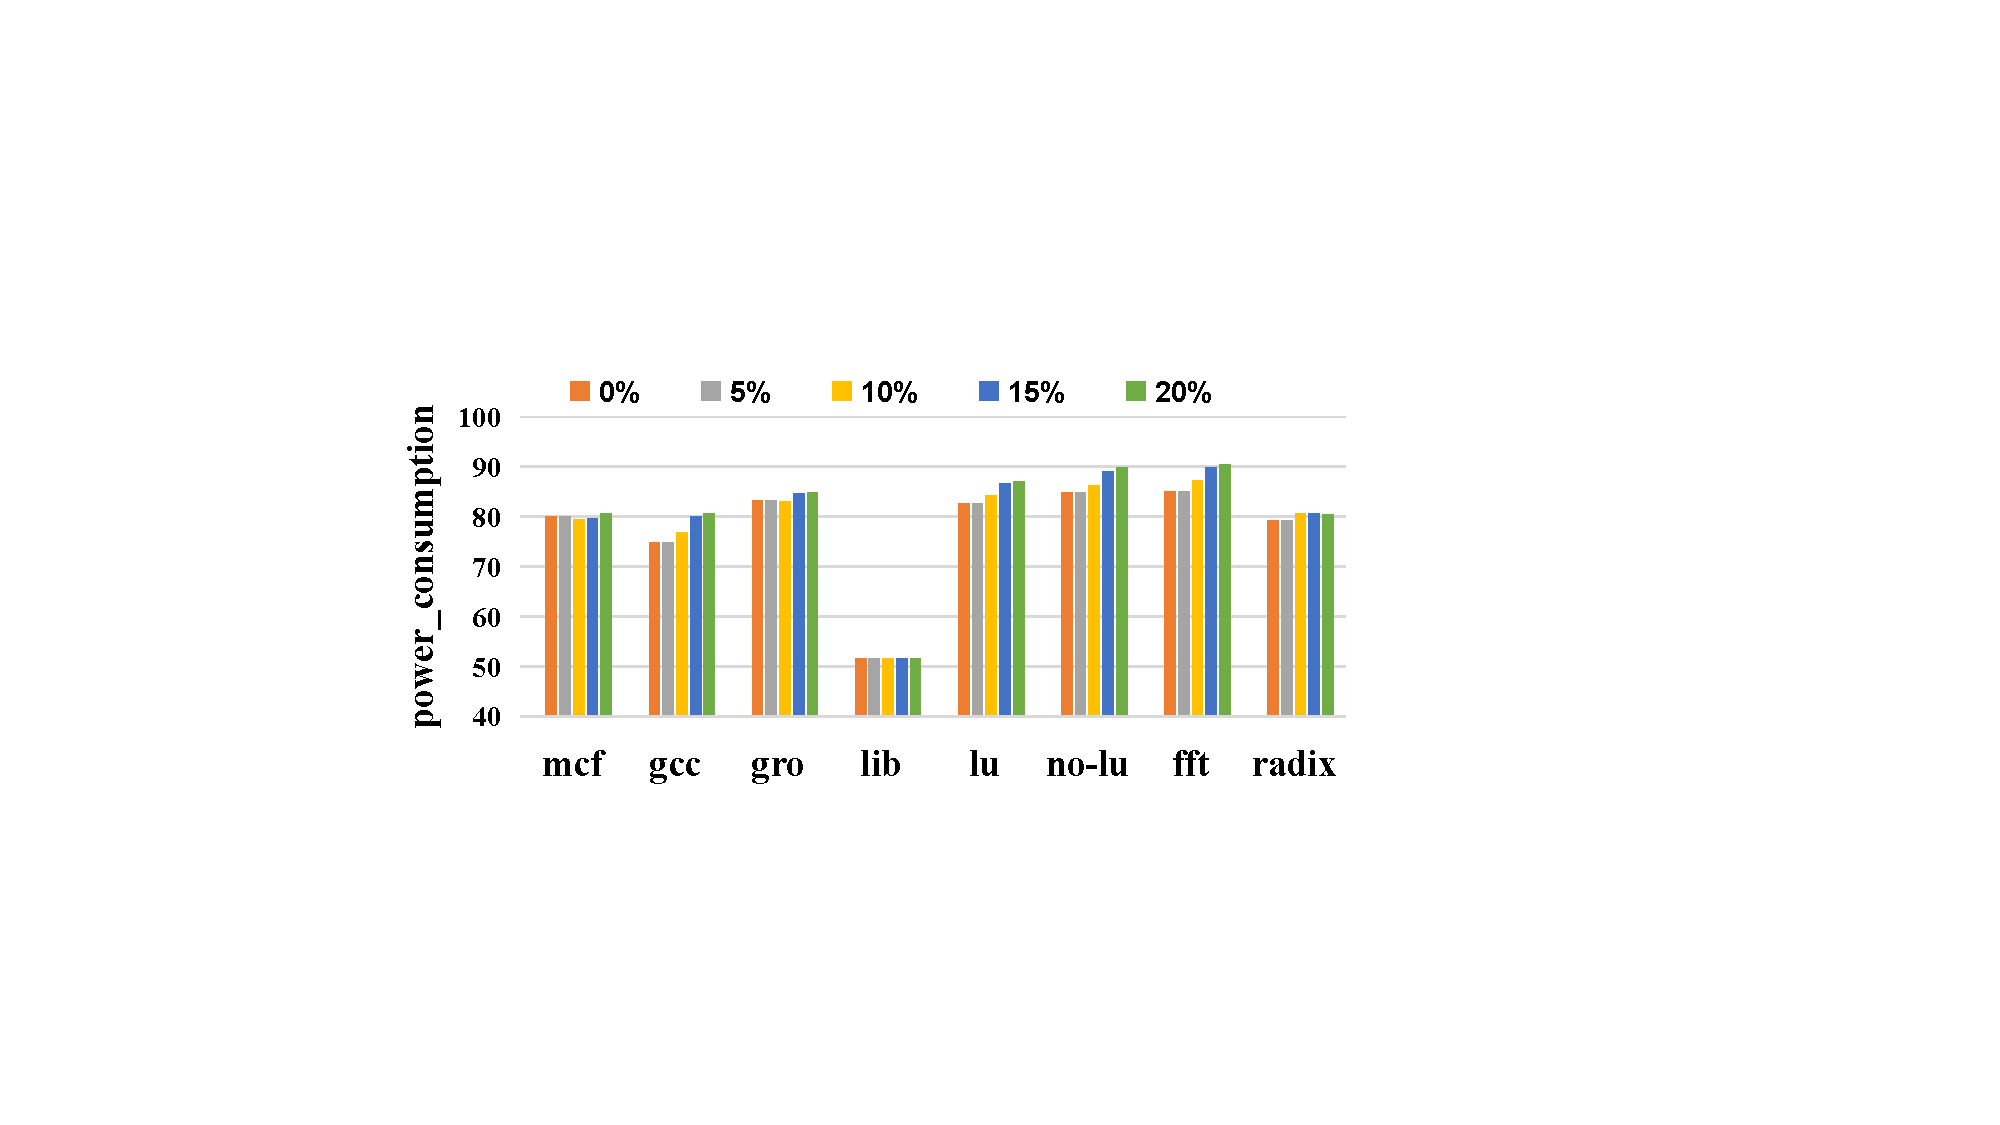
\includegraphics[width=0.92\linewidth]{thes_c}}
    \caption{CNT-Cache energy consumption distribution with different threshold.}
\label{fig:threshold-inc}
\vspace{-1em}
\end{figure}

CNT-Cache brings in both additional control logic and SRAM cells.
The increased SRAM cells are mainly used to store the access history 
of each cache line and the encoding direction. When the encoding granularity is set 
to be 64B and the encoding cycle is set to be 15, we need 8 bits to hold the cache 
line access counter and write counter, 1 bit for encoding direction. In addition, we also 
need FIFOs (depth 4) to store the encoded data as well as the cache line index. They 
take up the majority of the increased chip area and induce 2.21\% chip area overhead.
Compared to these storage components, the encoding logic and the predictor consumes 
much less chip area overhead, which is negligible according to our experiments.
